\subsubsection{ClientView}
\begin{enumerate}
	%- hier muss das PDF mit der Gesamtübersicht hin
	\item \textbf{\underline{MainActivity}}
	
	\begin{figure}[H]
		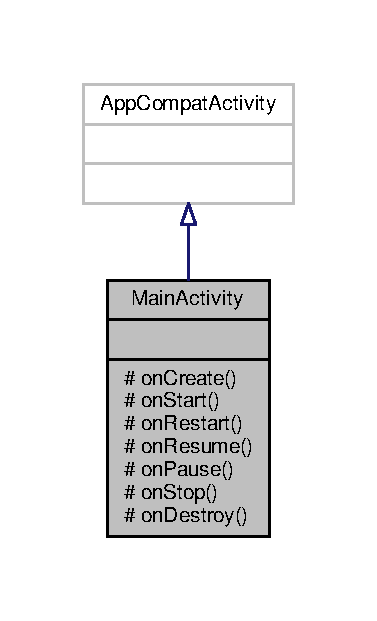
\includegraphics[scale = 1]{res/main_activity__inherit__graph.pdf}
		\centering
	\end{figure}
	Aufgrund der MVC Struktur der App ist die MainActivity die Hauptactivity des View Teil. Beim Öffnen der App auf dem Client wird diese als erste Activity geöffnet. Sie hat vor allem eine managende Funktion: sie überpfüft ob dieser Client schon registriert ist oder nicht. Sie erbt von der AppCompatActivity und implementiert dementsprechen auch deren Methoden.
	
	\textbf{Methoden}
	\begin{enumerate}
		\item protected onCreate(Bundle savedInstanceState) 
		
		Erweitert die onCreate Methode der AppCompatActivity indem sie, wenn der Client schon registriert ist, erst an die UsernameActivity weiterleitet. Ist er jedoch schon registriert, so leitet sie direkt an die zuletzt aufgerufene GroupActivity weiter.
		
		\item protected onStart()
		
		Erweitert die onStart() Methode der AppCompatActivity %- blabla ich habe keine Ahnung, was die wirklich macht
		
		\item protected onRestart()
		
		Erweitert die onRestart() Methode der AppCompatActivity %- blabla ich habe keine Ahnung, was die wirklich macht
		
		\item protected onResume()

		Erweitert die onResume() Methode der AppCompatActivity %- blabla ich habe keine Ahnung, was die wirklich macht
		
		\item protected onPause()

		Erweitert die onPause() Methode der AppCompatActivity %- blabla ich habe keine Ahnung, was die wirklich macht
		
		\item protected onStop()

		Erweitert die onStop() Methode der AppCompatActivity %- blabla ich habe keine Ahnung, was die wirklich macht
		
		\item protected onDestroy()

		Erweitert die onDesroy() Methode der AppCompatActivity %- blabla ich habe keine Ahnung, was die wirklich macht
	\end{enumerate}
	
	\item \textbf{\underline{UsernameActivity}}
	
	\begin{figure}[H]
		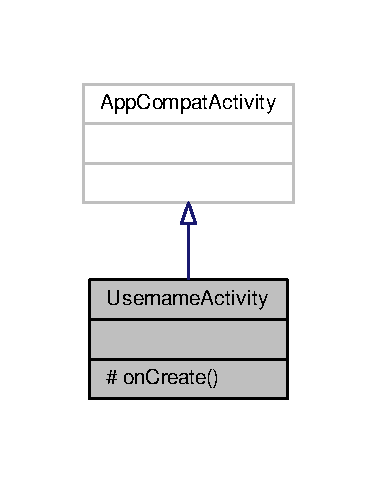
\includegraphics[scale = 1]{res/username_activity__inherit__graph.pdf}
		\centering
	\end{figure}
	Die UsernameActivity ist für das benennen des Benutzernamens zuständig. Sie wird sowohl zum ersten Start der App von der MainActivity aufgerufen, als auch von von der GroupActivity, wenn der Benutzer auf den Benutzernamen tippt. Sie enthält das UsernameChangeFragment und das UsernameRegistrationFragment. Sie erbt von der AppCompatActivity und implementiert dementsprechen auch deren Methoden.
	
	\textbf{Methoden}
	
	\begin{enumerate}
		\item protected onCreate(@Nullable Bundle savedInstanceState)
		
		Erweitert die onCreate Methode der AppCompatActivity mit dem laden des UsernameChangeFragments.
	\end{enumerate}
	
	\item \textbf{\underline{UsernameRegistrationFragment}}
	
	\begin{figure}[H]
		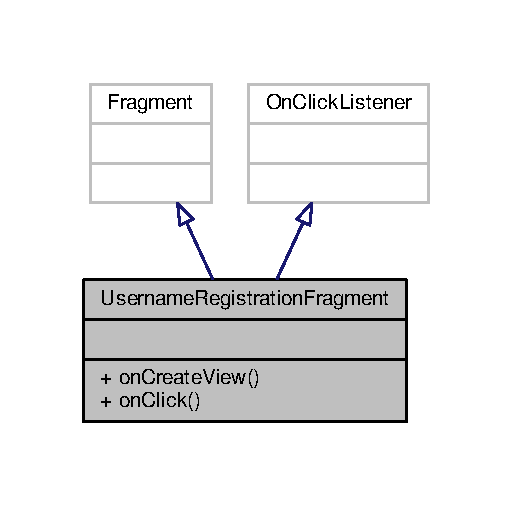
\includegraphics[scale = 1]{res/username_registration_fragment__inherit__graph.pdf}
		\centering
	\end{figure}
	Das UsernameRegistrationFragment ist dafür zuständig einen neuen User auf dem Server anzulegen. Es wird auf jedem Client in den username\_container der UsernameActivity geladen und somit nur einmalig aufgerufen, bis sich der Benutzer registriert hat. Es legt die erste Ansicht fest, die ein Benutzer sieht, wenn er die App das erste mal öffnet, bzw. wenn er die App öffnet und sich noch nie registriert hat. Es erbt von Fragment und implementiert den View.onClickListener. Dementsprechend implementiert sie auch deren Methoden.
	
	\textbf{Methoden}
	
	\begin{enumerate}
		\item public onCreateView(LayoutInflater inflater, ViewGroup container, Bundle savedInstanceState): View

		Erweitert die onCreateView Methode des Fragments mit der gewünschten Ansicht, die der View übergeben wird und fürgt dem OnClickListener den Button hinzu. Diese Methode gibt die aktuelle View zurück.
		
		\item public onClick(View view)

		Implementiert die onClick Methode des OnClickListeners, so dass beim Klicken auf den Next-Button überprüft wird, ob der gewünschte Benutzername zugelassen ist. In diesem Fall legt er einen neuen User an und leitet an eine leere GroupActivity weiter.
	\end{enumerate}

	\item \textbf{\underline{UsernameChangeFragment}}
		
	\begin{figure}[H]
		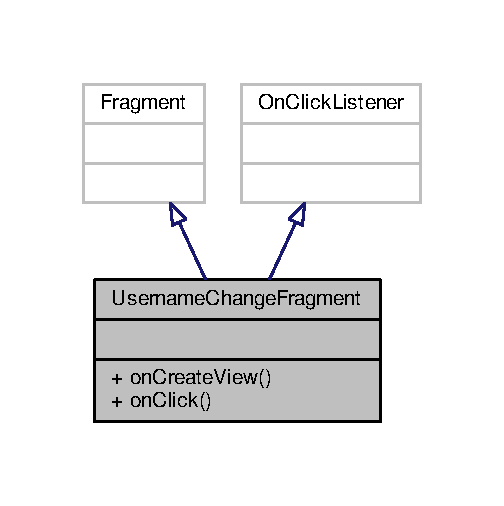
\includegraphics[scale = 1]{res/username_change_fragment__inherit__graph.pdf}
		\centering
	\end{figure}
	Das UsernameChangeFragment ist dafür zuständig den Username zu ändern. Es wird von der UsernameActivity in den username\_container geladen. Es legt die Ansicht fest, die ein Benutzer sieht, wenn er seinen Benutzernamen ändern möchte. Es erbt von Fragment und implementiert den View.onClickListener. Dementsprechend implementiert es auch deren Methoden.
	
	\textbf{Methoden}
	
	\begin{enumerate}
		\item public onCreateView(LayoutInflater inflater, ViewGroup container, Bundle savedInstanceState): View
		
		Erweitert die onCreateView Methode des Fragments mit der gewünschten Ansicht, die der View übergeben wird und fügt dem OnClickListener den Button hinzu, wenn der Benutzer die App nicht zum ersten Mal öffnet. In diesem Fall lädt es das UsernameRegistrationFragment in den username\_container der UsernameActivity. Diese Methode gibt die aktuelle View zurück.
		
		\item public onClick(View view)
		
		Implementiert die onClick Methode des OnClickListeners, so dass beim Klick auf dem Next-Button überprüft wird, ob der gewünschte neue Benutzername zugelassen ist. In diesem Fall ändert er diesen und leitet an die zuletzt aufgerufene GroupActivity weiter.
	\end{enumerate}
	
	\item \textbf{\underline{GroupActivity}}
	
	\begin{figure}[H]
		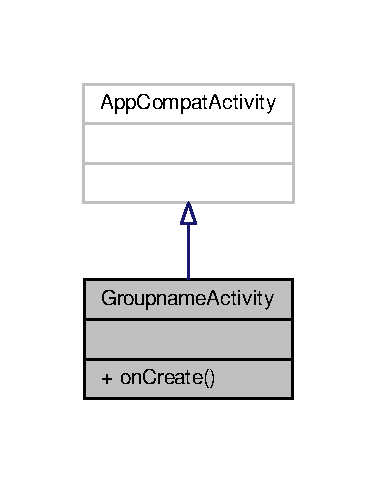
\includegraphics[scale = 1]{res/groupname_activity__inherit__graph.pdf}
		\centering
	\end{figure}
	GroupActivity ist für das Management der Gruppe zuständig. Sie ist die Activity, die die meiste Zeit geöffnet ist. Von allen anderen Activitys aus kann sie aus geöffnet werden. Sie enthält das GroupMapFragment, das GroupMapGoFragment und das GroupmembersFragment. Sie erbt von der AppCompatActivity und implementiert dementsprechen auch deren Methoden.
	
	\textbf{Methoden}
	
	\begin{enumerate}
		\item protected onCreate(@Nullable Bundle savedInstanceState

		Erweitert die onCreate Methode der AppCompatActivity mit dem laden des GroupMapFragments in den group\_container .
	\end{enumerate}
	
	\item \textbf{\underline{GroupMapFragment}}

	\begin{figure}[H]
		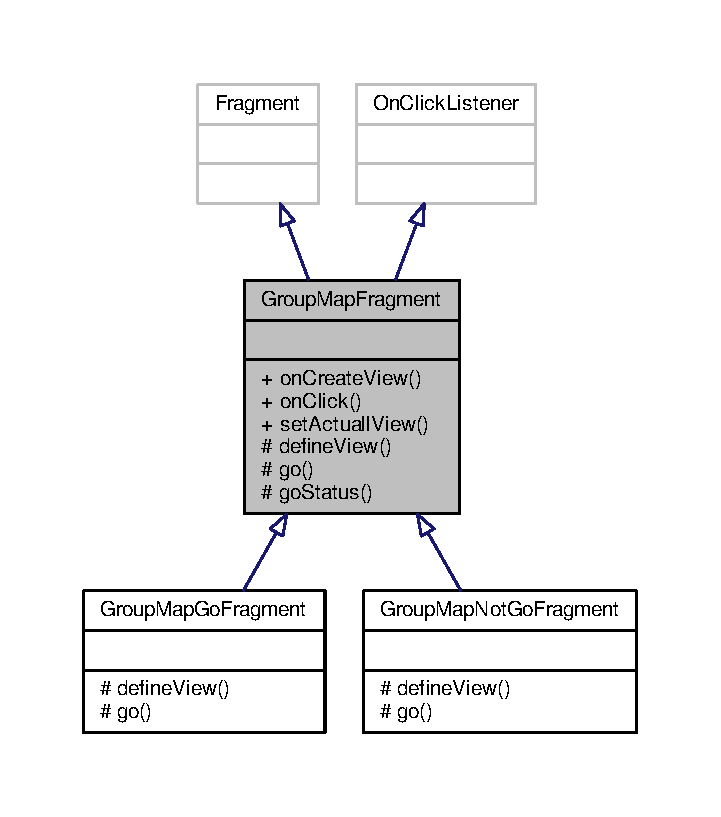
\includegraphics[scale = 1]{res/group_map_fragment__inherit__graph.pdf}
		\centering
	\end{figure}
	Das GroupMapFragment ist dafür zuständig, die Map-Ansicht anzuzeigen. Allerdings hat es lediglich die Funktion die Oberklasse für das GroupMapGoFragment und das GroupMapNotGoFragment zu sein, wird also niemals direkt aufgerufen. Es erbt von Fragment und implementiert den View.onClickListener. Dementsprechend implementiert es auch deren Methoden.
	
	\textbf{Methoden}	
	\begin{enumerate}
		\item public onCreateView(LayoutInflater inflater, ViewGroup container, Bundle savedInstanceState): View
		
		Erweitert die onCreateView Methode des Fragments mit der gewünschten Ansicht, indem es defineView() aufruft und den controller der MapView definiert. Außerdem fügt es dem OnClickListener die Button hinzu.Diese Methode gibt die aktuelle View zurück.
		
		\item protected defineView(LayoutInflater inflater, ViewGroup container): View

		Gibt die gewünschte View zurück. Allerdings ist diese Methode hier lediglich ein Platzhalter für detaillierte Methoden.
		
		\item public onClick(View view)
		
		Implementiert die onClick Methode des OnClickListeners, so dass er beim Klick auf den Gruppennamen das GroupMembersFragment in den group\_container der GroupActivity lädt, beim Klick auf das Datum, wenn man Gruppenadministrator ist, das GroupAppointmentFragment in den group\_container der GroupActivity lädt und beim Klick auf den Go-Button die go() Methode aufruft.
		
		\item protected go(MapView mapView)
		
		Definiert was passiert, wenn der Benutzer den Go-Button drückt. Allerdings ist diese Methode hier lediglich ein Platzhalter für detaillierte Methoden.
		
		\item public setActualView(IGeoPoint geoPoint, int newZoom)
		
		Speichert die aktuelle Zoom- und Fokus-Einstellung eines anderen GroupMapFragments
	\end{enumerate}
	
	\item \textbf{\underline{GroupMapNotGoFragment}}
	\begin{figure}[H]
		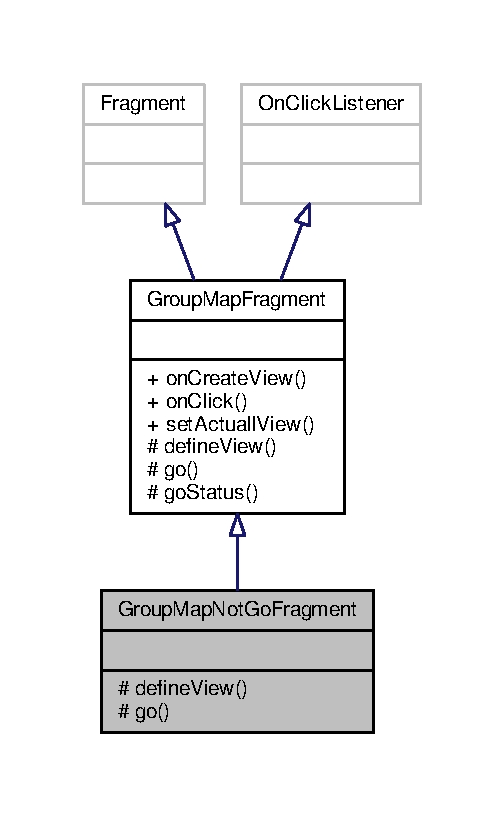
\includegraphics[scale = 1]{res/group_map_not_go_fragment__inherit__graph.pdf}
		\centering
	\end{figure}
	Das GroupMapNotGoFragment ist dafür zuständig, die Map-Ansicht anzuzeigen, wenn der Go-Button nicht gedrückt ist. Es wird von der GroupActivity in den group\_container geladen, immer dann wenn eine Gruppe aufgerufen wird. Es erbt von dem GroupMapFragment und implementiert dementsprechen auch dessen Methoden.
	
	\textbf{Methoden}	
	\begin{enumerate}
		
		\item protected defineView(LayoutInflater inflater, ViewGroup container): View

		Gibt die gewünschte View zurück. Wenn jedoch der Go-Button gedrückt ist, lädt es das GroupMapGoFragment in den group\_container der GroupActivity.
		
		\item protected go(MapView mapView)
		
		Lädt das GroupMapGoFragment in den group\_container der GroupActivity.
	\end{enumerate}
			
	\item \textbf{\underline{GroupMapGoFragmen}}

	\begin{figure}[H]
		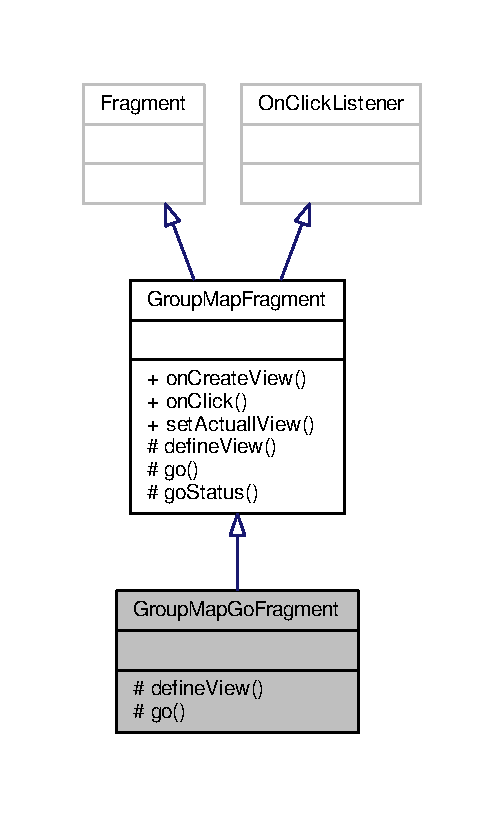
\includegraphics[scale = 1]{res/group_map_go_fragment__inherit__graph.pdf}
		\centering
	\end{figure}
		Das GroupMapGoFragment ist dafür zuständig, die Map-Ansicht anzuzeigen, wenn der Go Button gedrückt ist. In diesem Fall wird es von dem GroupMapNotGoFragment in den group\_container geladen, wenn der Benutzer go drückt, bzw. go gedrückt hat. Es erbt von dem GroupMapFragment und implementiert dementsprechend auch dessen Methoden.

	\textbf{Methoden}
	\begin{enumerate}
		\item protected defineView(LayoutInflater inflater, ViewGroup container): View

		Gibt die gewünschte View zurück.

		\item protected go(MapView mapView)

		Lädt das GroupMapNotGoFragment in den group\_container der GroupActivity.

	\end{enumerate}

	\item \textbf{\underline{GroupAppointmentFragment}}

	\begin{figure}[H]
		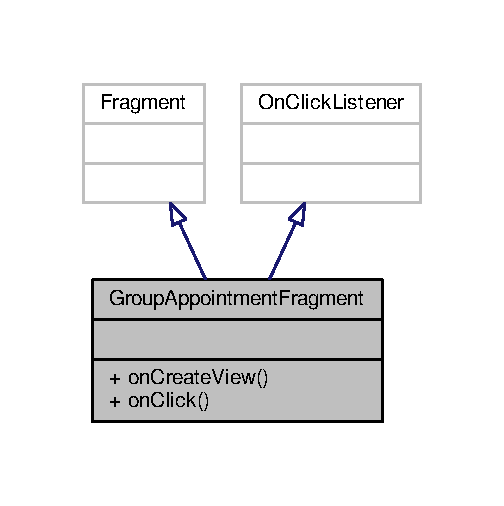
\includegraphics[scale = 1]{res/group_appointment_fragment__inherit__graph.pdf}
		\centering
	\end{figure}
	Das GroupAppointmentFragment ist dafür zuständig ein neues Treffen zu erstellen. Es wird von einem GroupFragment in den group\_container geladen, wenn der Gruppenadministrator auf den Appointment-Button drückt. Es erbt von Fragment und implementiert den View.onClickListener. Dementsprechend implementiert es auch deren Methoden.
	
	\textbf{Methoden}
	\begin{enumerate}
		\item public onCreateView(LayoutInflater inflater, @Nullable ViewGroup container, @Nullable Bundle savedInstanceState): View
			Gibt die gewünschte View zurück und fügt dem On.Click.Listener die Button hinzu.
			
		\item public onClick(View view)
		
		Implementiert die onClick Methode des OnClickListeners, so dass er beim Klick auf den Gruppennamen das GroupMembersFragment in den group\_container der GroupActivity lädt, beim Klick auf das Datum das GroupMapGoFragment, bzw. das GroupMapNotGoFragment in den group\_container der GroupActivity lädt, beim Klick auf die Time-, Date-, bzw. Place-Button das TimePickerFragment, DatePickerFragment, bzw. das GroupMapFragment lädt damit der Gruppenadministrator die Daten für ein Treffen auszuwählen und beim Klick auf den Next-Button dieses Appointment zu bestätigen kann. Dieses wird dann als nächstes Treffen in der Gruppe gespeichert.
		
	\end{enumerate}
	\item \textbf{\underline{TimePickerFragment}}

	\begin{figure}[H]
		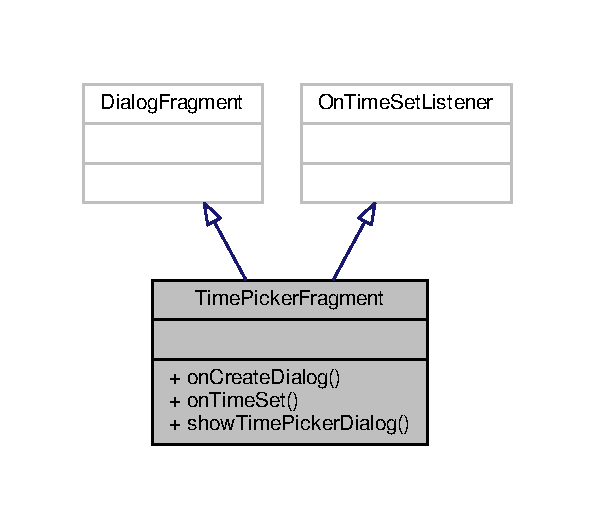
\includegraphics[scale = 1]{res/time_picker_fragment__inherit__graph.pdf}
		\centering
	\end{figure}
	Das TimePickerFragment ist dafür zuständig eine Uhrzeit auszuwählen und diese zurückzugeben. Es wird von dem GroupAppointmentFragment geladen, wenn der Benutzer den Time-Button drückt. Es erbt vom DialogFragment und implementiert den TimePickerDialog.OnTimeSetListener. Dementsprechend implementiert es auch deren Methoden.

	\textbf{Methoden}
	\begin{enumerate}
		\item public onCreateDialog(Bundle savedInstanceState): Dialog
	
		Öffnet den TimePickerDialog
		
		\item public onTimeSet(TimePicker view, int hourOfDay, int minute)
	
		Speichert die gewählte Zeit in einem gesonderten Appointment
		
		\item public showTimePickerDialog(View view)
		
		Macht den TimePickerDialog sichtbar
	\end{enumerate}
	\item \textbf{\underline{DatePickerFragment}}

	\begin{figure}[H]
		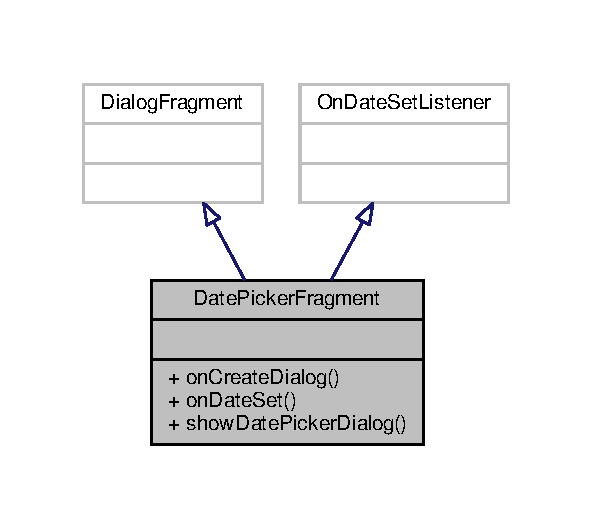
\includegraphics[scale = 1]{res/date_picker_fragment__inherit__graph.pdf}
		\centering
	\end{figure}
	Das DatePickerFragment ist dafür zuständig ein Datum auszuwählen und dieses zurückzugeben. Es wird von dem GroupAppointmentFragment geladen, wenn der Benutzer den Date-Button drückt. Es erbt vom DialogFragment und implementiert den DatePickerDialog.OnDateSetListener. Dementsprechend implementiert es auch deren Methoden.

	\textbf{Methoden}
	\begin{enumerate}
		\item public onCreateDialog(Bundle savedInstanceState): Dialog

		Öffnet den DatePickerDialog

		\item public onDateSet(DatePicker view, int year, int month, int day)

		Speichert das gewählte Datum in einem gesonderten Appointment

		\item public showDatePickerDialog(View view)

		Macht den DatePickerDialog sichtbar
	
	\end{enumerate}


	\item \textbf{\underline{GroupMembersFragment}}
	
	\begin{figure}[H]
		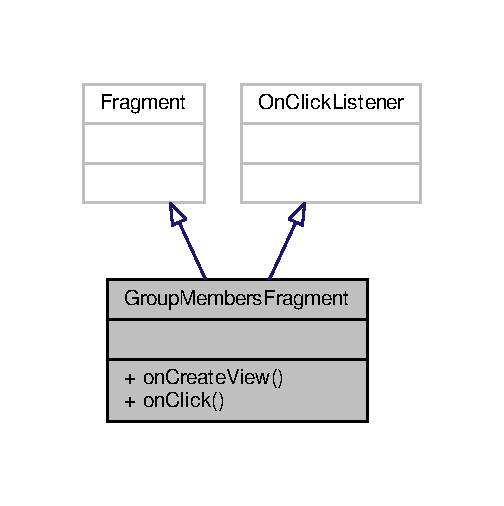
\includegraphics[scale = 1]{res/group_members_fragment__inherit__graph.pdf}
		\centering
	\end{figure}
	Das GroupMembersFragment ist dafür zuständig die Gruppenmitglieder zu verwalten. Es wird von einem GroupFragment in den group\_container geladen, wenn der Benutzer auf den Groupname-Button drückt. Es erbt von Fragment und implementiert den View.onClickListener. Dementsprechend implementiert es auch deren Methoden.
	
	\textbf{Methoden}
	\begin{enumerate}
		\item public onCreateView(LayoutInflater inflater, @Nullable ViewGroup container, @Nullable Bundle savedInstanceState): View
		
		Erweitert die onCreateView Methode des Fragments mit der gewünschten Ansicht, je nachdem ob der Benutzer Gruppenadministrator dieser Gruppe ist oder nicht. Außerdem kreiert es eine RecyclerView, ruft den MemberAdapter auf um alle Gruppenmitglieder anzeigen zu können und fügt der OnClickListener die Button hinzu.
		
		\item public onClick(View view)
		
		Implementiert die onClick Methode des OnClickListeners, so dass er beim Klick auf den Gruppennamen das GrouMapNotGoFragment, bzw. das GroupMapGoFragment in den group\_container der GroupActivity lädt, beim Klick auf das Datum das GroupAppointmentFragment, in den group\_container der GroupActivity lädt und beim Klick auf den AddMember-Button den SendLinkDialog lädt.
	\end{enumerate}
	\item \textbf{\underline{MemberAdapter}}

	\begin{figure}[H]
		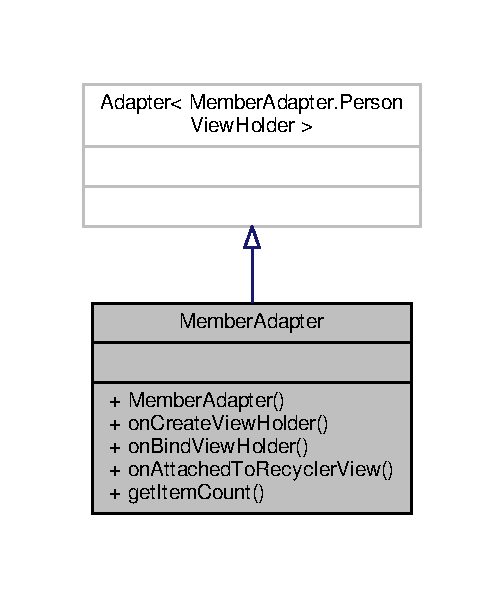
\includegraphics[scale = 1]{res/member_adapter__inherit__graph.pdf}
		\centering
	\end{figure}
	Der MemberAdapter hat die Aufgabe die Liste der Mitglieder in die RecyclerView zu laden. Er wird von dem GroupMembersFragment aufgerufen. Er erbt von RecyclerView.Adapter<MemberAdapter.PersonViewHolder> und implementiert dementsprechend auch dessen Methoden. Außerdem kreiert er die public static class PersonViewHolder, die von RecyclerView.ViewHolder erbt und dafür zuständig ist den Inhalt der RecyclerView zu speichern.

	\textbf{Methoden}
	\begin{enumerate}
		\item public MemberAdapter(int groupID)
		
		Stellt einen passenden Konstruktor bereit
		
		\item public PersonViewHolder onCreateViewHolder(ViewGroup parent, int viewType)
	
		Erstellt eine neue View, wenn sie vom LayoutManager aufgerufen wird
		
		\item public onBindViewHolder(PersonViewHolder holder, int i)

		Ersetzt den Inhalt der View, wenn sie vom LayoutManager aufgerufen wird
		
		\item public onAttachedToRecyclerView(RecyclerView recyclerView)
		
		Ruft die selbe Methode der Oberklasse auf
		
		\item public getItemCount(): int

		Gibt die Größe von dem Datensatz zurück, wenn sie vom LayoutManager aufgerufen wird
	\end{enumerate}


	\item \textbf{\underline{GroupnameActivity}}
	
	\begin{figure}[H]
		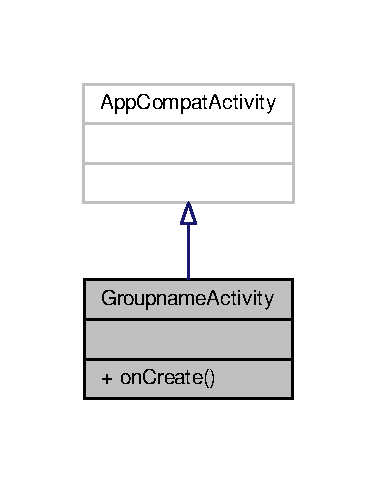
\includegraphics[scale = 1]{res/groupname_activity__inherit__graph.pdf}
		\centering
	\end{figure}
	Die GroupnameActivity ist für das Verwalten der Gruppe zuständig. Sie wird von einem GroupFragment aufgerufen, sowohl wenn der Benutzer den CreateGroup-Button drückt, als auch wenn ein Gruppenadministrator den Namen seiner Gruppe umbenennen will. Sie enthält das GroupnameChangeFragment und das GroupnameCreateFragment. Sie erbt von der AppCompatActivity und implementiert dementsprechen auch deren Methoden.
	
	\textbf{Methoden}
	\begin{enumerate}
		\item protected onCreate(@Nullable Bundle savedInstanceState)
		
		Erweitert die onCreate Methode der AppCompatActivity mit dem laden des GroupnameCreateFragments in den groupname\_container.
		
	\end{enumerate}
	
	\item \textbf{\underline{GroupnameChangeFragment}}
	
	\begin{figure}[H]
		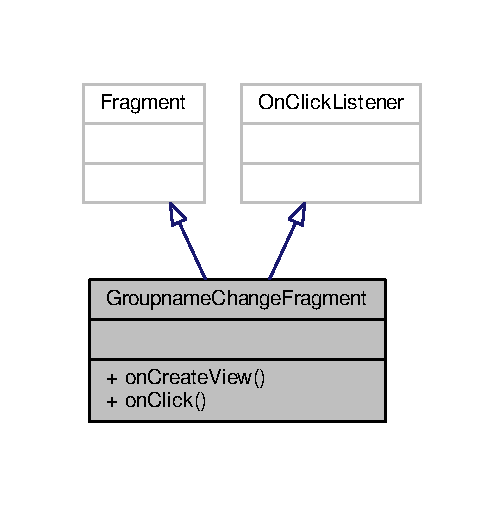
\includegraphics[scale = 1]{res/change_fragment__inherit__graph.pdf}
		\centering
	\end{figure}
	Das GroupnameChangeFragment ist dafür zuständig den Gruppenname zu ändern. Es wird von dem GroupnameCreateFragment in den groupname\_container geladen. Es legt die Ansicht fest, die ein Benutzer sieht, wenn er einen Gruppennamen ändern möchte. Es erbt von Fragment und implementiert den View.onClickListener. Dementsprechend implementiert es auch deren Methoden.
	
	\textbf{Methoden}	
	\begin{enumerate}
		\item public onCreateView(LayoutInflater inflater, ViewGroup container, Bundle savedInstanceState): View
		
		Erweitert die onCreateView Methode des Fragments mit der gewünschten Ansicht, die der View übergeben wird, fügt der View den alten Gruppennamen und dem OnClickListener den Button hinzu. Diese Methode gibt die aktuelle View zurück.
		
		\item public onClick(View view)
		
		Implementiert die onClick Methode des OnClickListeners, so dass beim Klick auf dem Next-Button überprüft wird, ob der gewünschte neue Gruppenname zugelassen ist. In diesem Fall ändert er diesen und leitet an dessen GroupActivity weiter.
	\end{enumerate}

	\item \textbf{\underline{GroupnameCreateFragment}}
	
	\begin{figure}[H]
		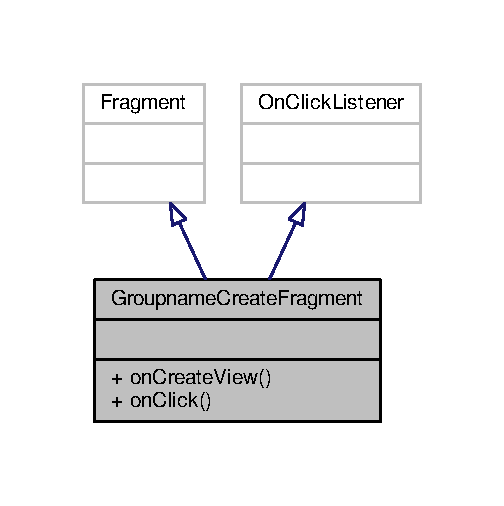
\includegraphics[scale = 1]{res/create_fragment__inherit__graph.pdf}
		\centering
	\end{figure}
	Das GroupnameCreateFragment ist dafür zuständig eine neue Gruppe auf dem Server anzulegen. Es legt die Ansicht fest, die ein Benutzer sieht, wenn er den CreateGroup-Button gedrückt hat. Es erbt von Fragment und implementiert den View.onClickListener. Dementsprechend implementiert sie auch deren Methoden.
	
	\textbf{Methoden}
	
	\begin{enumerate}
		\item public onCreateView(LayoutInflater inflater, ViewGroup container, Bundle savedInstanceState): View
		
		Erweitert die onCreateView Methode des Fragments mit der gewünschten Ansicht, die der View übergeben wird und fürgt dem OnClickListener den Button hinzu, wenn der Benutzer nicht eine bestehende Gruppe ausgewählt hat, in der er Administrator ist. In diesem Fall läd sie das GroupnameCreaterFragment in den groupname\_container. Diese Methode gibt die aktuelle View zurück.
		
		\item public onClick(View view)
		
		Implementiert die onClick Methode des OnClickListeners, so dass beim Klicken auf den Next-Button überprüft wird, ob der gewünschte Gruppenname zugelassen ist. In diesem Fall legt er eine neue Gruppe an und leitet an dessen GroupActivity weiter.
	\end{enumerate}

\end{enumerate}